\documentclass{article}


% if you need to pass options to natbib, use, e.g.:
%     \PassOptionsToPackage{numbers, compress}{natbib}
% before loading neurips_2023


% ready for submission
\usepackage[preprint]{neurips_2023}


% to compile a preprint version, e.g., for submission to arXiv, add add the
% [preprint] option:
%     \usepackage[preprint]{neurips_2023}


% to compile a camera-ready version, add the [final] option, e.g.:
%     \usepackage[final]{neurips_2023}


% to avoid loading the natbib package, add option nonatbib:
%    \usepackage[nonatbib]{neurips_2023}


\usepackage[utf8]{inputenc} % allow utf-8 input
\usepackage[T1]{fontenc}    % use 8-bit T1 fonts
\usepackage{hyperref}       % hyperlinks
\usepackage{url}            % simple URL typesetting
\usepackage{booktabs}       % professional-quality tables
\usepackage{amsfonts}       % blackboard math symbols
\usepackage{nicefrac}       % compact symbols for 1/2, etc.
\usepackage{microtype}      % microtypography
\usepackage{xcolor}         % colors
\usepackage{multirow}
\usepackage{graphicx}       % include images
\usepackage{caption}
\usepackage{algorithm}
\usepackage{algorithmic}
\usepackage{amsmath}
\usepackage{amssymb}
\usepackage{amsthm}
\usepackage{enumitem}
\usepackage{bm}
% \usepackage{titlesec}
\usepackage{geometry}   
\newtheorem{definition}{Definition}
\newtheorem{lemma}{Lemma}
\newtheorem{proposition}{Proposition}
\newtheorem{theorem}{Theorem}


% Images folder


\title{Unsupervised Domain Adaptation}


% The \author macro works with any number of authors. There are two commands
% used to separate the names and addresses of multiple authors: \And and \AND.
%
% Using \And between authors leaves it to LaTeX to determine where to break the
% lines. Using \AND forces a line break at that point. So, if LaTeX puts 3 of 4
% authors names on the first line, and the last on the second line, try using
% \AND instead of \And before the third author name.


\author{ Krishna Agarwal\\%\thanks{Use footnote for providing further information
    %about author (webpage, alternative address)---\emph{not} for acknowledging
    %funding agencies.} \\
  Indian Institute of Science, Bangalore\\
  \texttt{krishnaagarw@iisc.ac.in} \\
  % examples of more authors
   \And
  {Pratham Gupta} \\
  Indian Institute of Science, Bangalore\\
  \texttt{prathamgupta@iisc.ac.in} \\
   \And
   {Gavish Bansal} \\
   Indian Institute of Science, Bangalore\\
   \texttt{gavishbansal@iisc.ac.in} \\
   \And
   {Kintan Saha} \\
   Indian Institute of Science, Bangalore\\
   \texttt{kintansaha@iisc.ac.in} \\
  % \And
  % Coauthor \\
  % Affiliation \\
  % Address \\
  % \texttt{email} \\
}


\begin{document}
\graphicspath{{./images/}}

\maketitle


\begin{abstract}
  Traditional supervised deep learning assumes that training and test data share the same distribution—an assumption often violated in real-world scenarios. Domain adaptation addresses this issue. In this report, we focus on Unsupervised Domain Adaptation (UDA), where only the source domain is labeled. We implement and evaluate several deep UDA algorithms on benchmark datasets and compare our results with those from the original papers.
\end{abstract}


\section{Introduction}
Unsupervised Domain Adaptation (UDA) addresses the challenge of training models on a labelled source domain and adapting them to an unlabeled target domain with a different data distribution. In this report, we explore state-of-the-art UDA techniques and their applications in areas such as computer vision and natural language processing. We also reproduce results from influential works \cite{ganin2016domainadversarialtrainingneuralnetworks,survey,Ben-David2010} to deepen our understanding of this field. Our code is available at\footnote{\href{https://github.com/PrathamGupta423/unsupervised_domain_adaptation.git}{https://github.com/PrathamGupta423/unsupervised\_domain\_adaptation.git}}.


\section{Methodology}

\subsection{Algorithms}
We have implemented the following algorithms for our experiments:[For more details refer appendix]
\begin{itemize}
  \item \textbf{DANN (Domain-Adversarial Neural Network)}\cite{ganin2016domainadversarialtrainingneuralnetworks}: Trains the model in an adversarial manner to learn the domain invariant features using a gradient reversal layer and a DNN.
  \item \textbf{CORAL (Correlation Alignment), DeepCORAL}\cite{Coral,DeepCoral}: CORAL aligns the second-order statistics (covariances) of source and target features. Accordingly, DeepCORAL is an extension of CORAL that integrates correlation alignment into deep neural networks.
  \item \textbf{MMD (Maximum Mean Discrepancy)}\cite{sutherland2017generative}: A metric that quantifies non-alignment between the source and target distributions. It can be used as a loss function for DNNs.
  \item \textbf{DSN (Domain Separation Network)}\cite{DSN}: Separates domain-specific and domain-invariant features for better adaptation. A state of the art method for domain invariant feature learning.
  \item \textbf{ATT (Adversarial Training with Triplet loss)}\cite{pmlr-v70-saito17a}:An ensemble method that utilize two classifier trained on source domain to pseudo-label target domain to learn a classifier for it.
\end{itemize}

\subsection{Datasets}
We have used the following datasets\ref{tab:datasets} for our experiments:
\begin{table}
  \centering
  \caption{Benchmark datasets used in our experiments.}
  \label{tab:datasets}
  \begin{tabular}{ll}
      \toprule
      \textbf{Dataset Category} & \textbf{Datasets} \\
      \midrule
      Computer Vision (Numbers | Categorical)     & MNIST, MNIST-M, SVHN | Office: Amazon, DSLR, Webca \\
      % Computer Vision (Categorical) & Office: Amazon, DSLR, Webcam \\
      Sentiment Analysis (Classification)  & Amazon Review Sentiment \\
      \bottomrule
  \end{tabular}
\end{table}


\section{Experiments}


\subsection{Domain Adversarial Neural Networks (DANN)}
We implemented the DANN\cite{ganin2016domainadversarialtrainingneuralnetworks} architecture and evaluated it on a half-moon dataset, comparing it with a standard DNN. DANN showed poorer domain classification[Figures \ref{fig:vanilla},\ref{fig:dann}], indicating it learns more domain-invariant features.
We also tested DANN on the Amazon Reviews dataset using the paper’s architecture, training for 1000 epochs. Results closely match the paper (within 5\% deviation), with DANN generally outperforming other methods (Table \ref{tab:DANN_Sentiment}). We also test DANN on MNIST and MNIST-M Dataset and obtained results in accordance to the paper (88\% accuracy on target dataset [\ref{fig:dann_mnist_tar}] compared to only 60\% accuracy by doing source-only training\ref{fig:dann_mnist_source})

\begin{figure}
\centering
\begin{minipage}{0.32\linewidth}
\centering
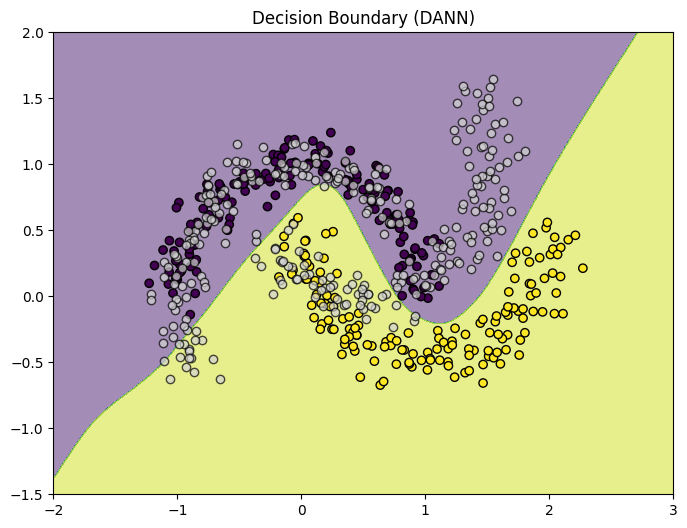
\includegraphics[width=0.7\linewidth]{DANN/label_decision_vanilla.png}
\caption{\small Label Classification}
\label{fig:label_decision_vanilla}
\end{minipage}
\hfill
\begin{minipage}{0.32\linewidth}
\centering
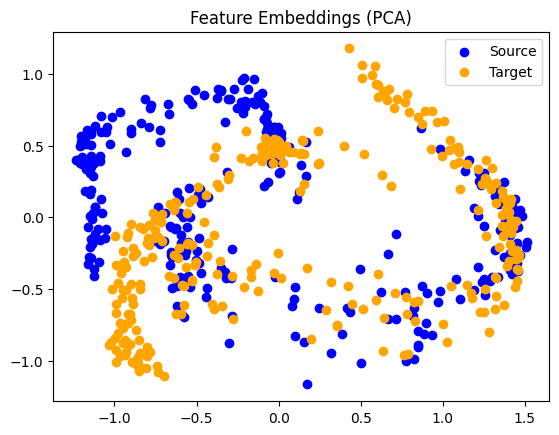
\includegraphics[width=0.7\linewidth]{DANN/feature_vanilla.png}
\caption{\small PCA of hidden layer}
\label{fig:feature_vanilla}
\end{minipage}
\hfill
\begin{minipage}{0.32\linewidth}
\centering
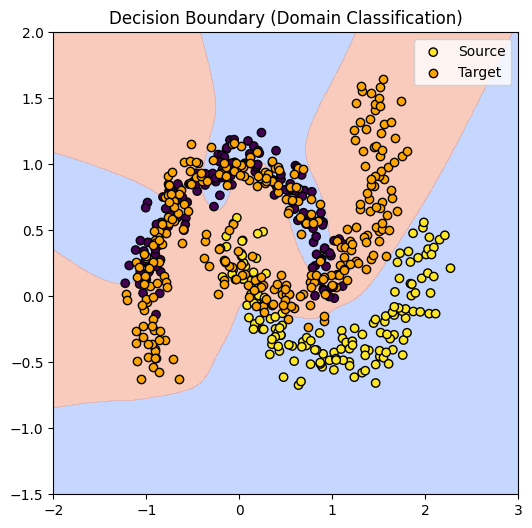
\includegraphics[width=0.55\linewidth]{DANN/domain_deciison_vanilla.png}
\caption{\small Domain Classification}
\label{fig:domain_decision_vanilla}
\end{minipage}
\caption{\small Results for Standard NN}
\label{fig:vanilla}
\end{figure}

\begin{figure}
\centering
\begin{minipage}{0.32\linewidth}
\centering
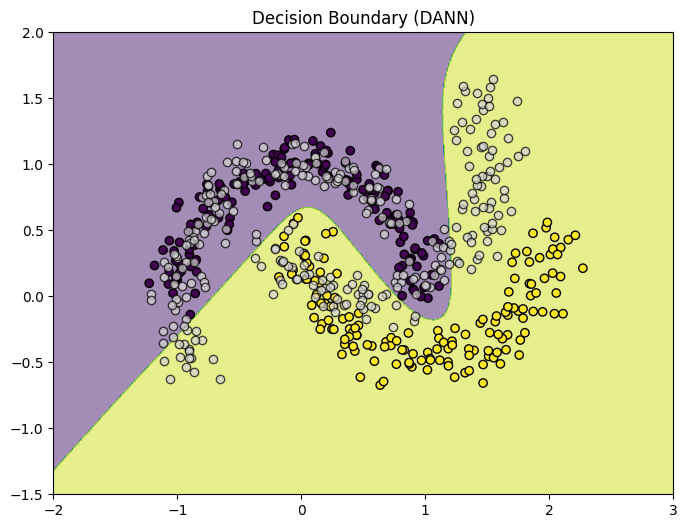
\includegraphics[width=0.7\linewidth]{DANN/label_decision_dann.png}
\caption{\small Label Classification}
\label{fig:label_decision_dann}
\end{minipage}
\hfill
\begin{minipage}{0.32\linewidth}
\centering
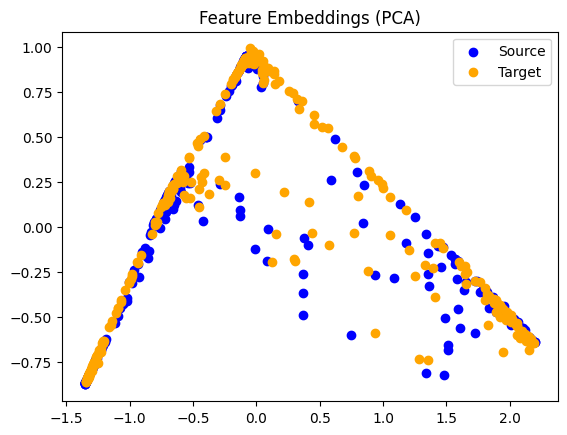
\includegraphics[width=0.7\linewidth]{DANN/feature_dann.png}
\caption{\small PCA of hidden layer}
\label{fig:feature_dann}
\end{minipage}
\hfill
\begin{minipage}{0.32\linewidth}
\centering
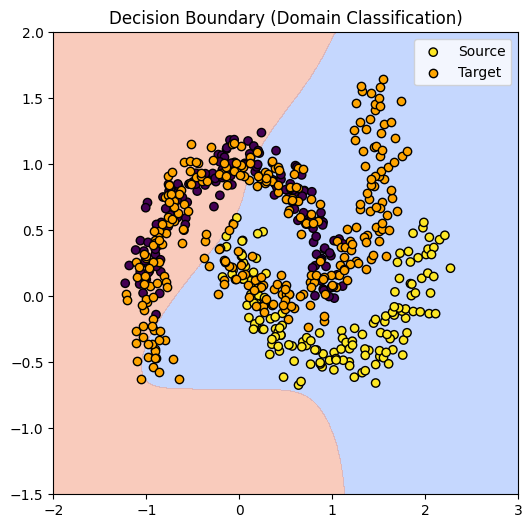
\includegraphics[width=0.55\linewidth]{DANN/domain_decision_dann.png}
\caption{\small Domain Classification}
\label{fig:domain_decision_dann}
\end{minipage}
\caption{\small Results for DANN}
\label{fig:dann}
\end{figure}

\begin{table}[t]
  \centering
  \caption{Results of DANN, NN, and SVM on Amazon Review Dataset compared with results reported in the paper.}
  \label{tab:DANN_Sentiment}
  \begin{tabular}{llcccccc}
    \toprule
    Source & Target & DANN & NN & SVM & DANN(p) & NN(p) & SVM(p) \\
    \midrule
    books & dvd         & \textbf{72.8}\% & \textbf{72.8}\% & 71.95\% & 78.4\% & 79.0\% & \textbf{79.9}\% \\
    books & electronics & \textbf{70.9}\% & 69.5\% & 69.5\% & 73.3\% & 74.7\% & \textbf{74.8}\% \\
    books & kitchen     & \textbf{71.85}\% & \textbf{71.85}\% & 71.7\% & \textbf{77.9}\% & 77.8\% & 76.9\% \\
    dvd   & books       & \textbf{71.55}\% & 66.9\% & 69\% & 72.3\% & 72.0\% & \textbf{74.3}\% \\
    dvd   & electronics & \textbf{69.8}\% & 69\% & 66.63\% & \textbf{75.4}\% & 73.2\% & 74.8\% \\
    dvd   & kitchen     & \textbf{70.05}\% & 67.25\% & 69.5\% & \textbf{78.3}\% & 77.8\% & 74.6\% \\
    electronics & books       & \textbf{65.95}\% & 63.8\% & 65.45\% & \textbf{71.3}\% & 70.9\% & 70.5\% \\
    electronics & dvd         & \textbf{68.05}\% & 67.15\% & 67\% & \textbf{73.8}\% & 73.3\% & 72.6\% \\
    electronics & kitchen     & \textbf{79.25}\% & 78.45\% & 78.75\% & \textbf{85.4}\% & \textbf{85.4}\% & 84.7\% \\
    kitchen & books       & 68.25\% & \textbf{68.75}\% & 68.05\% & \textbf{70.9}\% & 70.8\% & 70.7\% \\
    kitchen & dvd         & \textbf{68.90}\% & 65.15\% & 68.5\% & \textbf{74.0}\% & 73.9\% & 73.6\% \\
    kitchen & electronics & 78.75\% & 77.4\% & \textbf{79.25}\% & \textbf{84.3}\% & 84.1\% & 84.2\% \\
    \bottomrule
  \end{tabular}
\end{table}

\subsection{CORAL and DeepCORAL}

CORAL\cite{Coral} was implemented and tested for basic robustness by synthetic linearly separable random Gaussian datasets with same and different covariances. Results are reported in table\ref{tab:coral}.We also implemented the DeepCORAL\cite{DeepCoral} algorithm and observed its performance on the Office dataset. Our results alongwith the results mentioned in the survey paper[\cite{DeepCoral}] are shown in Table \ref{tab:deepcoral}. It is observable that the result for \textbf{W}$\rightarrow$ \textbf{A} is in slight disagreement of 4\% whose major reason we belive is hyperparameter mismatch and the training time of our implementation from the original approach.

\begin{table}
  \centering
  \caption{Performance of CORAL on synthetic datasets. Averaged over 100 iterations.}
  \label{tab:coral}
  \begin{tabular}{ccc}
    \toprule
    \textbf{Dataset Type} & \textbf{Covariance Condition} & \textbf{Accuracy (\%)} \\
    \midrule
    Univariate Random & Same Covariance & 100.0 \\
    Univariate Random & Different Covariance & 100.0 \\
    Multivariate Normal & Same Covariance & 95.80 \\
    Multivariate Normal & Different Covariance & 87.39 \\
    \bottomrule
  \end{tabular}
\end{table}

\begin{table*}
  \caption{Classification accuracy (source $\rightarrow$ target) of DeepCORAL on the Office computer vision dataset. A: Amazon, D: DSLR, W: Webcam.}
  \label{comparePerformance2}
  \begin{scriptsize}
  \begin{center}
  {\renewcommand{\arraystretch}{1.4}
  \begin{tabular}{@{}l cccccc@{}}
  \toprule
  \multicolumn{1}{c}{\multirow{2}{*}{\textbf{Result Source}}} & \multicolumn{6}{c}{\textbf{Office (Amazon, DSLR, Webcam)}} \\
  \cmidrule{2-7}
   & \textbf{A $\rightarrow$ W} & \textbf{D $\rightarrow$ W} & \textbf{W $\rightarrow$ D} & \textbf{A $\rightarrow$ D} & \textbf{D $\rightarrow$ A} & \textbf{W $\rightarrow$ A} \\
  \midrule
  \textbf{Our Code} & 62.05 & 95.32 & 99.56 & 64.44 & 52.77 & 56.49\\
  \hline
  \textbf{Survey Paper} & 66.4$\pm$0.4 & 95.7$\pm$0.3 & 99.2$\pm$0.1 & 66.8$\pm$0.6 & 52.8$\pm$0.2 & 51.5$\pm$0.3\\
  \bottomrule
  \end{tabular}
  }
  \end{center}
  \end{scriptsize}
  \label{tab:deepcoral}
\end{table*}

\subsection{Maximum Mean Discrepancy}
Similar to DeepCORAL\cite{DeepCoral}, We experimented with MMD\cite{sutherland2017generative} as the divergence metric. We using synthetic datasets and MMD showed strong adaptation ability (Fig \ref{fig:mmd}). 

\begin{figure}
  \centering
  \begin{minipage}{0.3\textwidth}
    \centering
    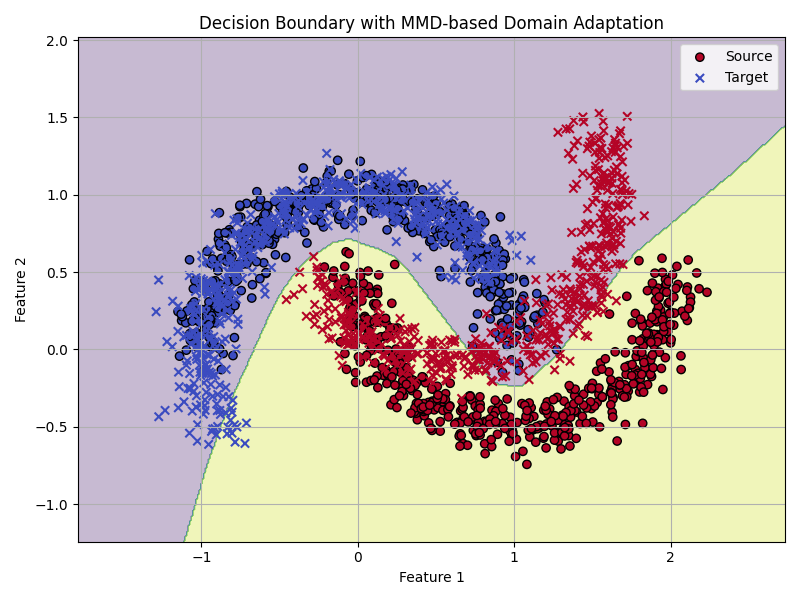
\includegraphics[width=\textwidth]{MMD/adaptation.png}
    \caption{Plot of desicion boundary of DNN trained with MMD loss. The decision boundary is shown for the source domain (dots) and target domain (cross).}
    \label{fig:mmd}
  \end{minipage}
  \hfill
  \begin{minipage}{0.3\textwidth}
    \centering
    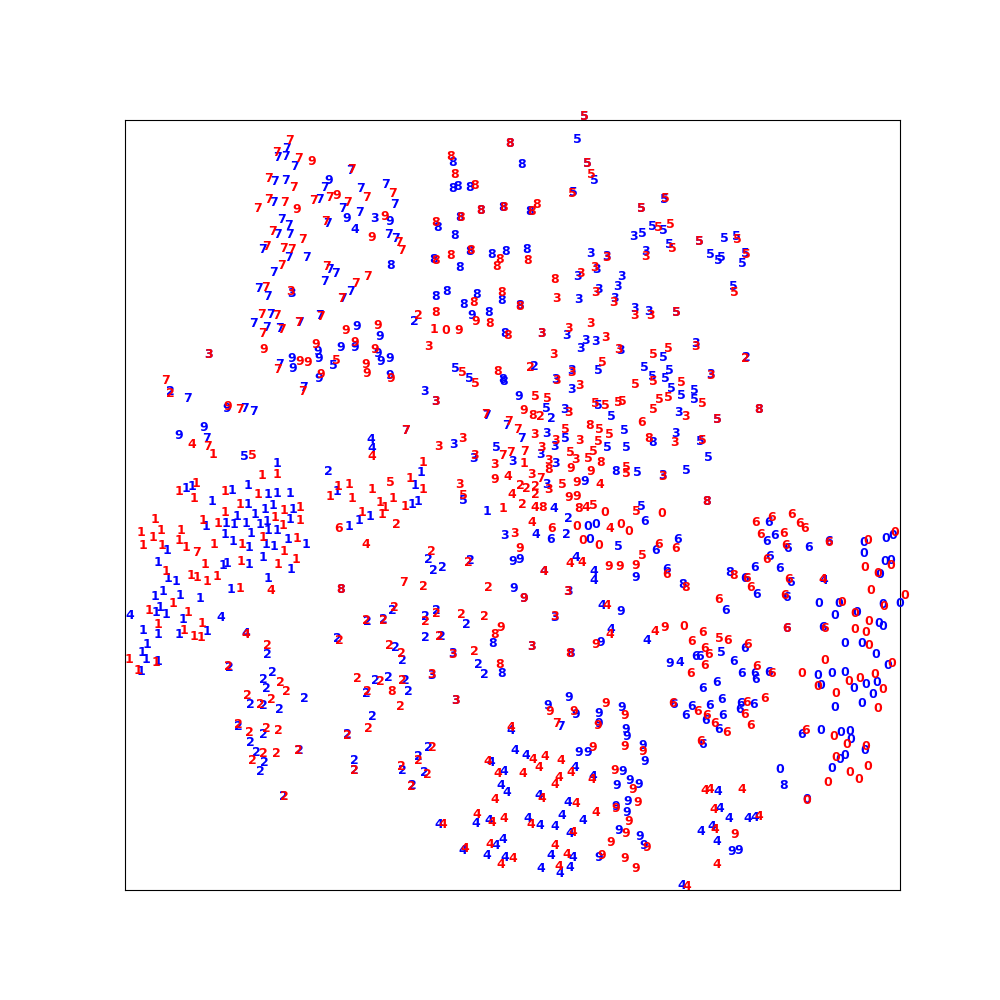
\includegraphics[width=\textwidth]{DANN/DANN.png}
    \caption{t-SNE Plot of features of Source and Target (With DANN)}
    \label{fig:dann_mnist_tar}
  \end{minipage}
  \hfill
  \begin{minipage}{0.3\textwidth}
    \centering
    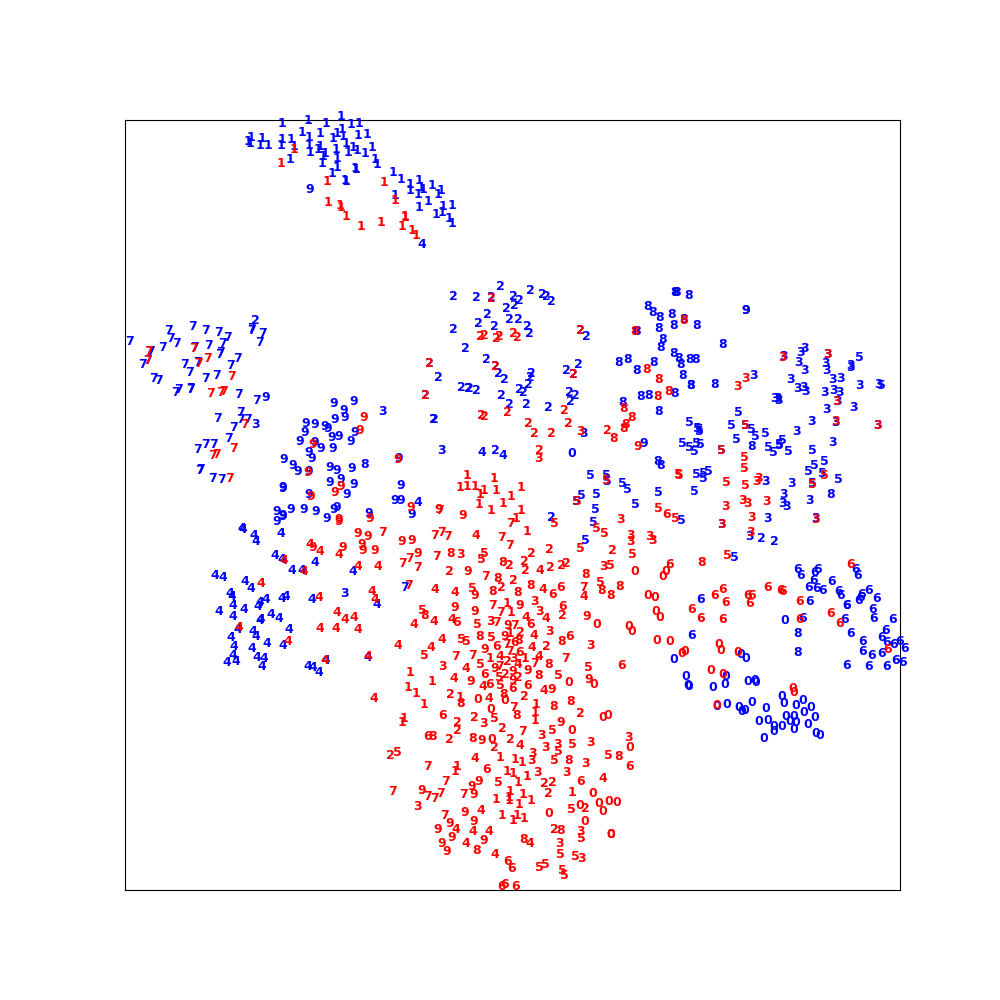
\includegraphics[width=\textwidth]{DANN/Source-only.png}
    \caption{t-SNE Plot of features of Source and Target (Without DANN)}
    \label{fig:dann_mnist_source}
  \end{minipage}
  

\end{figure}

\subsection{Domain Separation Network}
We implemented the DSN\cite{DSN} algorithm for domain adaptation on MNIST and MNIST-M. The accuracy (Table \ref{tab:dsn}) is comparable to the original paper, and reconstructed images are shown in Figure \ref{fig:dsn_reconstruction}.


\begin{figure}
  \centering
  % First minipage: the table
  \begin{minipage}[t]{0.45\textwidth}
    \centering
    \begin{minipage}[t]{0.95\textwidth}
      \centering
      \captionof{table}{Results of DSN on MNIST and MNIST-M Domain Adaptation.}
      \label{tab:dsn}
      \begin{tabular}{lc}
        \toprule
        \textbf{Method} & \textbf{Accuracy} \\
        \midrule
        DSN (Ours) & 81.6\% \\
        DSN (Paper) & 83.2\% \\
        \bottomrule
      \end{tabular}
    \end{minipage}
    \vspace{2mm}
    \begin{minipage}[t]{0.95\textwidth}
      \vspace{4mm}
      \centering
      \begin{minipage}[t]{0.95\textwidth}
        \centering
        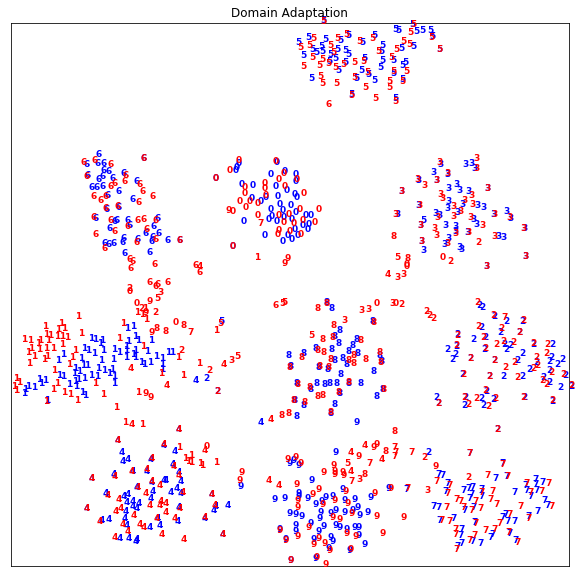
\includegraphics[width=0.6
        \linewidth]{DSN/DNS_MNIST_MNISTM.png}
        \caption{TSNE visualization for the DSN Experiment}
      \end{minipage}
    \end{minipage}
  \end{minipage}%
  \hfill
  % Second minipage: the 2x2 image grid
  \begin{minipage}[t]{0.5\textwidth}
    \caption{Reconstructed images from DSN.}
    \label{fig:dsn_reconstruction}
    \centering
    \begin{minipage}[t]{0.48\textwidth}
      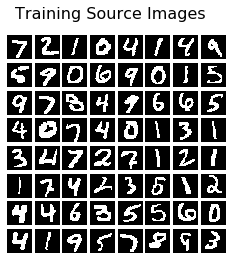
\includegraphics[width=0.85\linewidth]{DSN/source.png}
    \end{minipage}
    \hfill
    \begin{minipage}[t]{0.48\textwidth}
      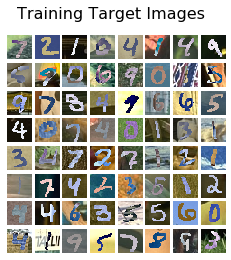
\includegraphics[width=0.85\linewidth]{DSN/target.png}
    \end{minipage}
    \vspace{2mm}
    \begin{minipage}[t]{0.48\textwidth}
      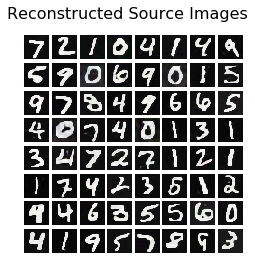
\includegraphics[width=0.9\linewidth]{DSN/reconstructed_source.png}
    \end{minipage}
    \hfill
    \begin{minipage}[t]{0.48\textwidth}
      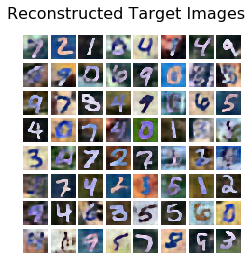
\includegraphics[width=0.9\linewidth]{DSN/reconstructed_target.png}
    \end{minipage}

  \end{minipage}
\end{figure}




\subsection{Asymmetric Tri-training for Unsupervised Domain Adaptation}
We implemented the Asymmetric Tri-Training\cite{pmlr-v70-saito17a}  algorithm and tested it on MNIST and SVHN. Results (Table \ref{tab:att_results}) are comparable to the paper's for the training without batch normalization. Discrepancies in other settings may be due to limited training time and suboptimal hyperparameter tuning.
\begin{table}
  \centering
  \caption{Results of ATT on MNIST and SVHN Domain Adaptation.}
  \label{tab:att_results}
  \begin{tabular}{lccc}
      \toprule
      \textbf{Method} & \textbf{MNIST\(\to\)SVHN} & \textbf{SVHN \(\to\) MNIST} \\
      \midrule
      Our w/o Batch Normalization & 36.9\% & 76.8\% \\
      Ours w/o Multi-view Loss & 15.2\% & 76.5\% \\
      Ours  & 15.2\% & 71.4\% \\
      \midrule
      Papers w/o Batch Normalization & 39.8\% & 79.8\% \\
      Papers w/o Multi-view Loss & 49.7\% & 86.0\% \\
      Papers  & 52.8\% & 85.8\% \\
      \bottomrule
  \end{tabular}
\end{table}





% \begin{figure}[h]
%   \centering
%   \includegraphics[width=0.5\textwidth]{ATT_Architecture.png}
%   \caption{ATT Architecture: The feature extractor F takes input from both source and target domain. F1 and F2 are classifiers trained on source domain. Ft is trained on target domain using pseudo-labels from F1 and F2.}
%   \label{fig:att_architecture}
% \end{figure}



\section{Conclusion}
In this report, we explored and implemented several state-of-the-art unsupervised domain adaptation algorithms across diverse datasets. Our results largely align with those reported in original works, validating both the effectiveness of these methods and our understanding of the underlying principles. This study highlights the importance of domain-invariant representations and provides a foundation for further research in robust model generalization across domains.



\newpage
\section{Appendix}


\subsection{Introduction}

A common issue in many machine learning applications arises when the distribution of the training data (source domain) differs from the test data (target domain). This phenomenon, known as \textbf{domain} shift, can severely degrade model performance. 

\textbf{Domain adaptation} is a subfield of transfer learning that aims to tackle this problem. Specifically, we will be dealing with Unsupervised domain adaptation. In this setting we will have access to:
\begin{itemize}[noitemsep]
    \item A labeled source domain \( \mathcal{D}_S \) with distribution \( P_S(X, Y) \),
    \item An unlabeled target domain \( \mathcal{D}_T \) with distribution \( P_T(X, Y) \),
\end{itemize}
where \( P_S(X, Y) \neq P_T(X, Y) \). The goal is to learn a model that performs well on \( \mathcal{D}_T \), using labels only from \( \mathcal{D}_S \).

% \section{Domain Adaptation Theory}

% Ben-David et al. (2006, 2010) proposed a generalization bound that directly motivates the DANN framework.

% \subsection{Generalization Bound}

% Let \( h \in \mathcal{H} \) be a hypothesis and let \( \epsilon_T(h) \) and \( \epsilon_S(h) \) be the expected classification errors on target and source domains respectively. Then:

% \begin{equation}
% \epsilon_T(h) \leq \epsilon_S(h) + \frac{1}{2} d_{\mathcal{H}\Delta\mathcal{H}}(\mathcal{D}_S, \mathcal{D}_T) + \lambda,
% \label{eq:gen-bound}
% \end{equation}

% where:
% \begin{itemize}[noitemsep]
%     \item \( d_{\mathcal{H}\Delta\mathcal{H}} \) is the symmetric difference hypothesis divergence.
%     \item \( \lambda = \min_{h \in \mathcal{H}} \left[ \epsilon_S(h) + \epsilon_T(h) \right] \).
% \end{itemize}

% This bound suggests that to achieve good performance on the target domain, one should:
% \begin{enumerate}[label=(\alph*)]
%     \item Minimize the source risk \( \epsilon_S(h) \),
%     \item Minimize the divergence between the domains.
% \end{enumerate}

\subsection{$\mathcal{H}$-Divergence and Proxy A-Distance}

We wish to measure the distances between domains, specifically our source domain and our target domain. Hence, we require a metric to measure the distances between domains. $\mathcal{H}$-Divergence is a metric which can be easily estimated from empirical data. Hence, $\mathcal{H}$-Divergence is our metric of choice.

\subsubsection{$\mathcal{H}$-Divergence}

Let \( \mathcal{H} \) be a hypothesis class of binary classifiers. The $\mathcal{H}$-Divergence between two marginal distributions \( \mathcal{D}_S^X \) and \( \mathcal{D}_T^X \) is defined as:

\begin{equation}
d_{\mathcal{H}}(\mathcal{D}_S^X, \mathcal{D}_T^X) = 2 \sup_{h \in \mathcal{H}} \left| \Pr_{x \sim \mathcal{D}_S^X}[h(x) = 1] - \Pr_{x \sim \mathcal{D}_T^X}[h(x) = 1] \right|.
\end{equation}

For a symmetric hypothesis class $\mathcal{H}$( a symmetric hypothesis class is one in which if $\eta$ is a classifier in hypothesis class then $1 - \eta$ is also a classifier in the hypothesis class), one can compute the \textit{empirical} $\mathcal{H}$-\textit{divergence} between two samples $S \sim (\mathcal{D}_S^X)^n$ and $T \sim (\mathcal{D}_T^X)^{n'}$(of sizes n and n' respectively) using the following:

\begin{equation}
\hat{d}_{\mathcal{H}}(S, T) = 2 \left( 1 - \min_{\eta \in \mathcal{H}} \left[ \frac{1}{n} \sum_{i=1}^{n} \mathbb{I}\left[\eta(x_i) = 0\right] + \frac{1}{n'} \sum_{i=n+1}^{N} \mathbb{I}\left[\eta(x_i) = 1\right] \right] \right),
\end{equation}

\subsubsection{Proxy A-Distance (PAD)}

Computing the exact empirical H-divergence is difficult, hence it is estimated via the \textbf{Proxy A-distance}:

\begin{equation}
\hat{d_A} = 2(1 - 2\epsilon),
\end{equation}
where \( \epsilon \) is the generalization error of a classifier trained to distinguish source from target domain samples.
\\
We will further see in discussion of "A Theory of learning from different domains" paper that this empirical bound for $\mathcal{H}$-Divergence converges to actual value as number of datapoints increases.

Having laid the theoretical groundwork, we'll now introduce the DANN architecture.



\subsection{Domain-Adversarial Neural Network (DANN)}

DANN incorporates a domain classifier into the neural network and trains the feature extractor to predict domain invariant features by continuous feedback(in terms of gradient) by a gradient reversal layer and simultaneously train on source dataset to learn the actual labels.

\subsubsection{Architecture}

The DANN consists of three components:
\begin{enumerate}[noitemsep]
    \item A feature extractor \( G_f(x; \theta_f) \),
    \item A label predictor \( G_y(G_f(x); \theta_y) \),
    \item A domain classifier \( G_d(G_f(x); \theta_d) \).
\end{enumerate}

\begin{center}
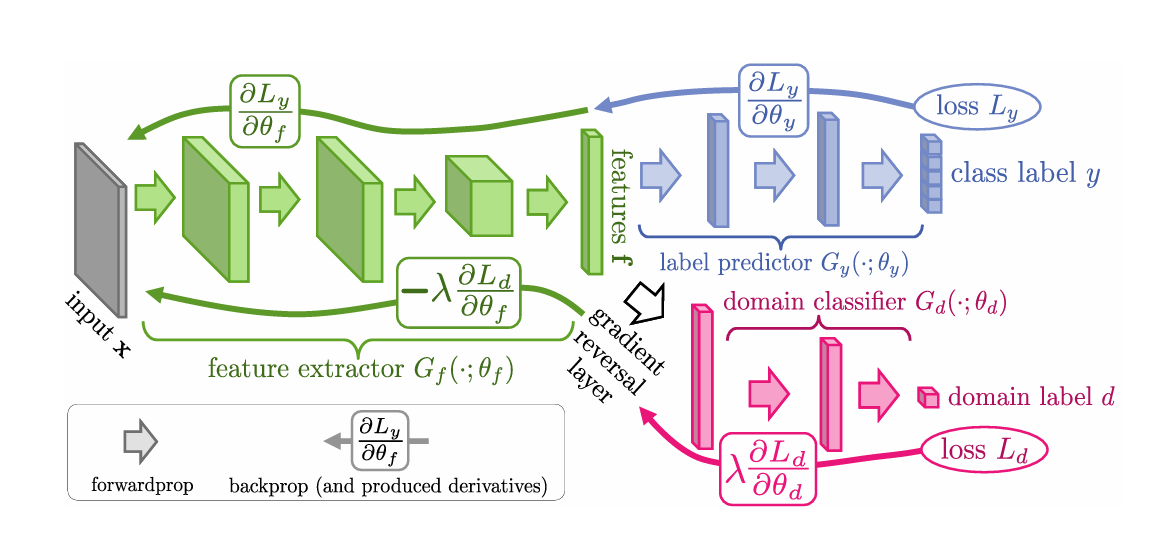
\includegraphics[width=0.8\textwidth]{DANN/DANN_img.png}
\end{center}

\textbf{Optimization Objective}

We define a joint loss:

\begin{align}
E(\theta_f, \theta_y, \theta_d) &= \frac{1}{n} \sum_{i=1}^{n} \mathcal{L}_y(G_y(G_f(x_i^s)), y_i^s) \nonumber \\
&\quad - \lambda \left( \frac{1}{n} \sum_{i=1}^{n} \mathcal{L}_d(G_d(G_f(x_i^s)), 0) + \frac{1}{m} \sum_{j=1}^{m} \mathcal{L}_d(G_d(G_f(x_j^t)), 1) \right).
\label{eq:objective}
\end{align}

This results in a saddle point problem:
\begin{align}
(\hat{\theta}_f, \hat{\theta}_y) &= \arg \min_{\theta_f, \theta_y} E(\theta_f, \theta_y, \hat{\theta}_d), \\
\hat{\theta}_d &= \arg \max_{\theta_d} E(\hat{\theta}_f, \hat{\theta}_y, \theta_d).
\end{align}

The first update is to learn domain invariant features and the required classifier whereas the second update is to learn domain classifier.

\textbf{Gradient Updates}

Using stochastic gradient descent, the updates are:

\begin{align}
\theta_f &\leftarrow \theta_f - \mu \left( \frac{\partial \mathcal{L}_y}{\partial \theta_f} - \lambda \frac{\partial \mathcal{L}_d}{\partial \theta_f} \right), \\
\theta_y &\leftarrow \theta_y - \mu \frac{\partial \mathcal{L}_y}{\partial \theta_y}, \\
\theta_d &\leftarrow \theta_d - \mu \lambda \frac{\partial \mathcal{L}_d}{\partial \theta_d}.
\end{align}

\subsubsection{Gradient Reversal Layer Working}

To simplify implementation, the adversarial optimization is performed via a custom layer called the Gradient Reversal Layer (GRL).

\subsubsubsection{Definition}

Let \( R(x) \) denote the GRL. It has the following behavior:
\begin{align}
\text{Forward pass:} \quad &R(x) = x, \\
\text{Backward pass:} \quad &\frac{dR}{dx} = -\lambda I.
\end{align}

During backpropagation, GRL multiplies the gradient by \(-\lambda\), reversing the gradient direction and forcing the feature extractor to generate domain-invariant features.

\begin{figure}[H]
    \centering
    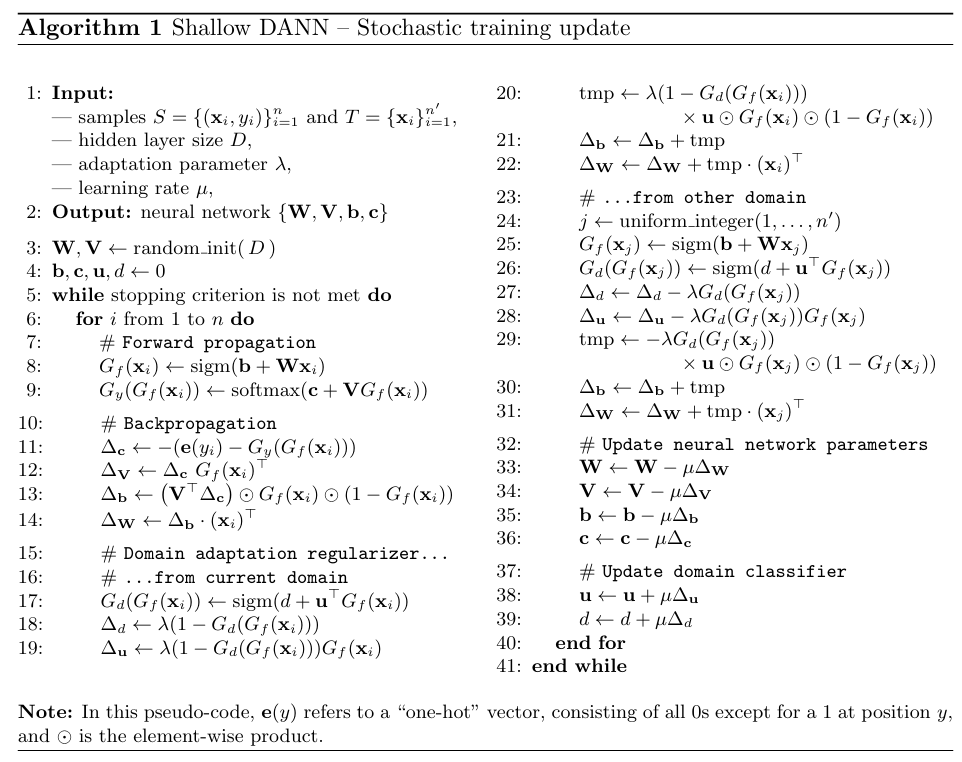
\includegraphics[width=1\linewidth]{images/DANN/ALGO.png}
    \caption{Pseudocode for the DANN architecture on a shallow neural network having 1 hidden layer of 15 neurons}
    \label{fig:enter-label}
\end{figure}

\subsubsection{Theoretical Implications}

DANN effectively minimizes the upper bound of the Target Error which will be discussed in the "A Theory of learning from different domains" paper. Through the adversarial training:
\begin{itemize}[noitemsep]
    \item The source classification loss \( \epsilon_S \) is minimized.
    \item The domain classifier's inability to distinguish domains results in low \( d_{\mathcal{H}\Delta\mathcal{H}} \).
\end{itemize}

Thus, for low values of \( \lambda \), DANN is expected to generalize well on the target domain.


\subsubsection{Under-performing Experiments}
We've encountered a persistent issue in our experiments on person re-identification using deep image descriptors. While most of our experiments have yielded promising results, one specific setup is consistently underperforming.

This particular experiment focuses on adapting a model trained on the PRiM dataset to the ViPER dataset. The core task is to learn a representation (embedding) of person images such that images of the same person, even when captured by different cameras, from varying viewpoints, and at different times, have similar embeddings.

Our approach involves the following:

\begin{enumerate}
    \item \textbf{Embedding Learning:} We train a deep neural network to generate image embeddings.
    \item \textbf{Similarity Measurement:} We calculate the cosine similarity between the embeddings of image pairs within a batch of size $n$. This results in an $n \times n$ similarity matrix.
    \item \textbf{Ground Truth Comparison:} We compare this similarity matrix with a ground truth matrix of the same size. The $(i, j)^{th}$ element of the ground truth matrix is 1 if the $i^{th}$ and $j^{th}$ images in the batch belong to the same person, and 0 otherwise.
    \item \textbf{Loss Function:} We use the Binomial Deviance Loss to quantify the discrepancy between the predicted similarity matrix and the ground truth matrix. Additionally, we incorporate a Cross-Entropy Loss to handle domain classification, aiming to make the learned features domain-invariant.
    \item \textbf{Optimization:} We use backpropagation to update the network's parameters based on the combined loss.
\end{enumerate}

However, we've observed a rather frustrating issue: the domain classification loss stops updating significantly after a certain number of training steps. We initially suspected the ReLU activation function might be the cause due to its zero gradient for negative inputs. To address this, we replaced ReLU with the Tanh activation function. Unfortunately, this change did not consistently resolve the issue of the domain loss stagnating.

Subsequently, we experimented with several architectural modifications and hyperparameter adjustments, including increasing the number of layers and trying different hyperparameter settings. We even replaced the split network structure with a fully connected layer. Furthermore, we explored alternative loss functions. Despite these efforts, we have not yet achieved satisfactory results for this specific adaptation task.

\subsubsection{Successful Experiments}
The effectiveness of the DANN (Domain Adversarial Neural Network) architecture has been validated through several key experiments.

\textbf{Intertwining-Moon Experiment:}
The first successful experiment involved a synthetic "intertwining-moons" dataset. A labeled source domain dataset was created, and an unlabeled target domain dataset was generated by rotating the source domain points by $35^\circ$. The performance of DANN was compared to a standard Neural Network (NN). The underlying neural network architecture being used is a shallow neural network having a single hidden layer of 15 neurons. Observing the label classification boundaries revealed that DANN's decision boundary not only classified the source labels effectively but also aligned with the structure of the rotated target data. Furthermore, Principal Component Analysis (PCA) visualization of the hidden layer representations showed that DANN successfully embedded the target and source domain features within each other, indicating the learning of domain-invariant features. In contrast, the standard DNN's hidden layer representation showed the target domain features clustering separately, near the boundaries of the source feature space. Similar domain invariance was observed in the domain classification features learned by DANN.
\\
\\
The dataset being considered can be found in Figure 14. The models were trained for 10000 epochs. Other training parameters have been taken from the paper. The results obtained via DANN can be found in Figure 8 and the results obtained by the standard DNN can be found in Figure 4. DANN has a domain accuracy \textbf{51.33\%} whereas our standard NN has a domain accuracy of \textbf{74.5\%}. This elucidates the fact that DANN tries to increase the inaccuracy in correctly predicting the domain thus promoting the \textbf{learning of domain-invariant features}.
\begin{figure}
    \centering
    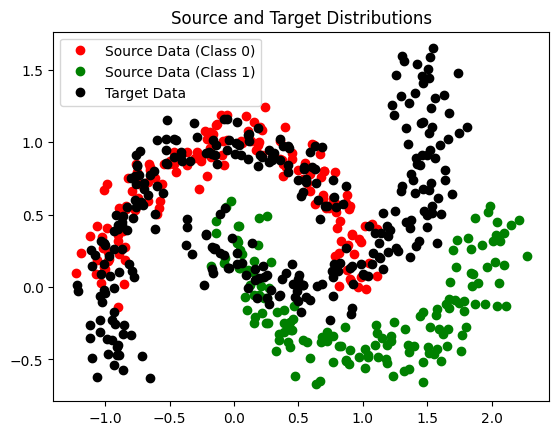
\includegraphics[width=0.5\linewidth]{images/DANN/moon.png}
    \caption{Half moons dataset}
    \label{fig:enter-label}
\end{figure}

\textbf{Sentiment Analysis on Amazon Reviews:}
The second experiment focused on sentiment analysis using the Amazon review dataset. This dataset comprises reviews across four different product domains: books, DVDs, electronics, and kitchen appliances. Data provided involve frequency of each word, pair of words and triplet of words from which we sampled out top 400 occurances in Source dataset as our Dictionary and the created a bag of words encoding for all datapoint to convert all them to a 400 dimentional vector. Domain adaptation was performed for every possible pair of these domains. The models were trained for 1000 epochs, and the results of DANN were compared against those of a standard Deep Neural Network (DNN) and Support Vector Machines (SVM). The study concluded that DANN generally outperformed both DNN and SVM across most of the domain transfer tasks, highlighting its ability to generalize sentiment classification across different product categories. The corresponding performance metrics were presented in a table\ref{tab:DANN_Sentiment} where out of 12 possible pairs of different source and target domains, a total of 10 pairs were giving their best results for DANN whereas 3 were giving their best results for DNN and 1 for SVM.

\textbf{MNIST to MNIST-M Adaptation:}
Finally, the paper presented a domain adaptation task involving the MNIST and MNIST-M datasets. MNIST contains grayscale images of handwritten digits, while MNIST-M is a modified version of MNIST with colored backgrounds and strokes resembling real-world images. The experiment demonstrated that DANN achieved the expected positive results in adapting a model trained on MNIST to classify images from the more challenging MNIST-M dataset. DANN produced a target accuracy of \textbf{88.03\% } whereas a model trained only on the source data produced a target accuracy of only \textbf{60.99\%}. The paper reports a target accuracy of \textbf{76.66\%} using DANN and a target accuracy of \textbf{56.90\%} without using DANN. The architecture used can be found in Figure 16.
\begin{figure}
    \centering
    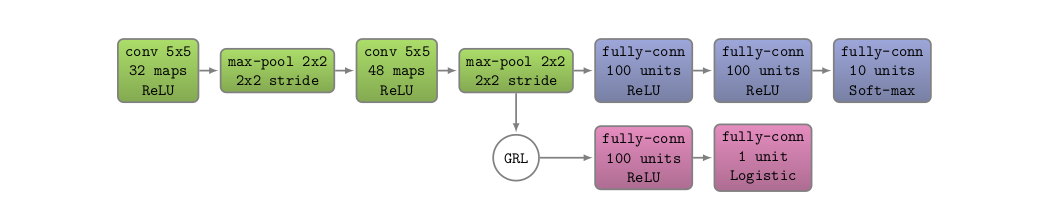
\includegraphics[width=0.8\linewidth]{images/DANN/mnist.png}
    \caption{MNIST DANN Architecture}
    \label{fig:enter-label}
\end{figure}
\\
\\
We also perform a t-SNE visualisation of the features given by the top feature extractor layer of the DANN network as well as the non-DANN network. The t-SNE visualisation was done with a perplexity parameter of 30. The visualisation can be found in Figures 10 and 11. We observe that the features of the source domain and the target domain learned by the DANN architecture are almost superimposed upon each other. This illustrates the fact that \textbf{DANN learns domain invariant features}. On the other hand, the visualisation of the source and target features for the non-DANN case shows that the features learnt are domain-dependent. 

\subsubsection{Conclusion}

The DANN framework stands as a principled and practical method for unsupervised domain adaptation. Grounded in domain adaptation theory, it achieves the minimization of target error by aligning feature distributions through adversarial training. The elegance of DANN lies in its simplicity and the minimal architectural modifications required to integrate domain adaptation directly into a standard feed-forward neural network.

\subsection{CORAL and DeepCORAL}
\subsubsection{Theory: CORAL}
CORAL is a divergence based method falling under Domain Invariant Feature Learning in which give the source data $\mathcal{D}_S$ and the target data $\mathcal{D}_T$, we tend to minimize the difference between the second order statistics(covariance matrices) of the train data and the test data for our classifier.

We describe our method by taking a multi-class classification problem as the running example. Suppose we are given source-domain training examples $D_S = \{\vec{x}_i\}$, $\vec{x} \in \mathbb{R}^D$ with labels $L_S = \{y_i\}, y \in \{1, \ldots, L\}$, and target data $D_T = \{\vec{u}_i\}, \vec{u} \in \mathbb{R}^D$. Here both $\vec{x}$ and $\vec{u}$ are the D-dimensional feature representations $\phi(I)$ of input $I$. Suppose $\mu_s, \mu_t$ and $C_S, C_T$ are the feature vector means and covariance matrices. As illustrated in Figure 2, $\mu_t = \mu_s = 0$ after feature normalization while $C_S \ne C_T$.

To minimize the distance between the second-order statistics (covariance) of the source and target features, we apply a linear transformation $A$ to the original source features and use the Frobenius norm as the matrix distance metric.

The multiplication of $A$ with the source data performs the tasks of whitening and recoloring the data to align it with the target domain.

\[
\min_A \|C'_S - C_T\|_F^2 = \min_A \|A^\top C_S A - C_T\|_F^2
\]

where $C'_S$ is covariance of the transformed source features $D_S A$ and $\|\cdot\|_F^2$ denotes the matrix Frobenius norm.

\subsubsection{Algorithm: CORAL}
Now, for all possible inequalities between the ranks of the source and target covariance matrices, we can analytically evaluate $A$ using singular value decomposition\cite{Coral}. However, since computing singular value decompositions of matrices is computationally heavy, we stick to traditional whitening and re-coloring.
The traditional whitening is adding a small regularization parameter $\lambda$ to the diagonal elements of the covariance matrix to explicitly make it full rank and then multiply the original feature by the inverse square root (or square root for coloring) of it. The whitening and re-coloring here are slightly different from them since the data are likely to lie on a lower-dimensional space and the covariance matrices could be low rank. For our experiments, we have set $\lambda$ to $1e-5$.

\subsubsection{Pseudocode: CORAL}

\begin{algorithm}[H]
\caption{CORAL}
\begin{algorithmic}[1]
\STATE \textbf{Input:} Source Data $D_S$, Target Data $D_T$, $\lambda$
\STATE \textbf{Output:} Adjusted Source Data $D_s^*$
\STATE $C_S = cov(D_S) + \lambda\cdot eye(size(D_S, 2))$
\STATE $C_T = cov(D_T) + \lambda\cdot eye(size(D_T, 2))$
\STATE $D_S = D_S * C_S^{-\frac{1}{2}}$        \%whitening source
\STATE $D_S^* = D_S*C_T^{\frac{1}{2}}$         \%re-coloring with target covariance
\end{algorithmic}
\end{algorithm}

\subsubsection{Theory: DeepCORAL}
We address the unsupervised domain adaptation scenario where there are no
labelled training data in the target domain, and propose to leverage both the
deep features pre-trained on a large generic domain
and the labelled source data. In the meantime, we also want the final learned
features to work well on the target domain. The first goal can be achieved by
initializing the network parameters from the generic pre-trained network and
fine-tuning it on the labelled source data. For the second goal, we propose to
minimize the difference in second-order statistics between the source and target
feature activations, i.e. the CORAL loss. Figure 1 shows a sample Deep CORAL
architecture using our proposed correlation alignment layer for deep domain
adaptation. We refer to Deep CORAL as any deep network incorporating the
CORAL loss for domain adaptation. And for our experiments we have used AlexNet as our network.

Basically, we assign some layers of our neural network to be the CORAL loss layers and fix the last layer as the Classification loss layer(in the multi-class classification setting). The basic skeleton of a DeepCORAL architecture has been shown in \ref{fig:deepcrl}

\begin{figure}[h]
  \centering
  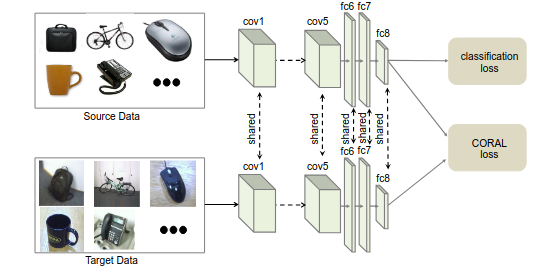
\includegraphics[width=0.8\textwidth]{images/DeepCORAL/DeepCORAL.png}
 \caption{A coarse skeleton of the DeepCORAL architecture. Both source and target data pass through a shared CNN feature extractor. The network minimizes a standard classification loss on source domain labels and a CORAL (CORrelation ALignment) loss to align second-order statistics (covariances) of source and target feature representations. Here we apply the CORAL loss to the $fc$8 layer of
AlexNet. Integrating it to other layers or network architectures should be straight-
forward. }
  \label{fig:deepcrl}
\end{figure}

\subsubsection{Mathematical Formulation: DeepCORAL}
We define the CORAL loss as the distance between the second-order statistics (covariances) of the source and target features(this is slightly different from the previous definition as now the source data for the next layer is the most recently aligned source data:
\[
\mathcal{L}_{\text{CORAL}} = \frac{1}{4d^2} \| C_S - C_T \|_F^2 \tag{1}
\]
where $\| \cdot \|_F$ denotes the squared matrix Frobenius norm. The covariance matrices of the source and target data are given by:
\[
C_S = \frac{1}{n_S - 1} \left( D_S^T D_S - \frac{1}{n_S} \left( \mathbf{1}^T D_S \right)^T \left( \mathbf{1}^T D_S \right) \right) \tag{2}
\]
\[
C_T = \frac{1}{n_T - 1} \left( D_T^T D_T - \frac{1}{n_T} \left( \mathbf{1}^T D_T \right)^T \left( \mathbf{1}^T D_T \right) \right) \tag{3}
\]
where $\mathbf{1}$ is a column vector with all elements equal to 1.

The gradient with respect to the input features can be calculated using the chain rule:
\[
\frac{\partial \mathcal{L}_{\text{CORAL}}}{\partial D_{ij}^S} = \frac{1}{d^2 (n_S - 1)} \left( \left( D_S^T - \frac{1}{n_S} \left( \mathbf{1}^T D_S \right)^T \mathbf{1}^T \right)^T (C_S - C_T) \right)_{ij} \tag{4}
\]
\[
\frac{\partial \mathcal{L}_{\text{CORAL}}}{\partial D_{ij}^T} = - \frac{1}{d^2 (n_T - 1)} \left( \left( D_T^T - \frac{1}{n_T} \left( \mathbf{1}^T D_T \right)^T \mathbf{1}^T \right)^T (C_S - C_T) \right)_{ij} \tag{5}
\]

We use batch covariances, and the network parameters are shared between two networks.

Hence, finally, our total loss to be minimized by training the neural network is as follows:
$$\mathcal{L} = \mathcal{L}_\text{CLASS} + \sum_{i=1}^{t} \lambda_i \mathcal{L}_{\text{CORAL}}$$
where $t$ is the number of CORAL loss layers.

\subsubsection{Experiments: DeepCORAL}
We used AlexNet as our pre-trained model in the experiments for DeepCORAL. The data used was the Office dataset and a discrepancy in the results obtained was highlighted earlier in the report which may be due to different hyperparameters set by us in comparison to the original experimental setup. We used SGD as our optimizer and trained the model over 50 epochs with a batch size of 128 and a step size(learning rate) of $1e-3$. The results for the experiments conducted by us are summarised in \ref{tab:deepcoral}.

\subsection{Maximum Mean Discrepancy}
\subsubsection{Theory}
Maximum Mean Discrepancy (MMD) is a statistical test used to measure the distance between two probability distributions. It is particularly useful in domain adaptation tasks where the goal is to align the feature distributions of the source and target domains. MMD computes the distance between the means of the two distributions in a reproducing kernel Hilbert space (RKHS). The MMD can be expressed mathematically as:
\[
  \text{MMD}^2(P, Q) = \left\| \frac{1}{m} \sum_{i=1}^{m} \phi(x_i) - \frac{1}{n} \sum_{j=1}^{n} \phi(y_j) \right\|^2_{\mathcal{H}}
\]
where \(P\) and \(Q\) are the two distributions, \(\phi\) is a feature map that maps the data into a high-dimensional space, and \(\mathcal{H}\) is the RKHS. The MMD can be computed using a kernel function, such as the Gaussian kernel, which allows for efficient computation in high-dimensional spaces. 
Formula for MMD is given as:
\[
  \text{MMD}^2(P, Q) = \mathbb{E}_{x,x'}[k(x,x')] + \mathbb{E}_{y,y'}[k(y,y')] - 2\mathbb{E}_{x,y}[k(x,y)]
\]
where \(k\) is the kernel function, and \(x\) and \(y\) are samples from the distributions \(P\) and \(Q\), respectively. 

An empirical estimate of MMD can be computed using the following formula:
\[
  \widehat{\text{MMD}}^2(P, Q) = \frac{1}{m(m-1)} \sum_{i=1}^{m} \sum_{j \neq i}^{m} k(x_i, x_j) + \frac{1}{n(n-1)} \sum_{i=1}^{n} \sum_{j \neq i}^{n} k(y_i, y_j) - \frac{2}{mn} \sum_{i=1}^{m} \sum_{j=1}^{n} k(x_i, y_j)\cite{JMLR:v13:gretton12a}
\]
From this we can define the test statistic as:
\[
  T = \frac{\widehat{\text{MMD}}^2(X,Y)}{\sqrt{\hat{V_m}(X,Y)}}
\]
where \(\widehat{V_m}(X,Y)\) is the variance of the MMD estimate. The null hypothesis is that the two distributions are equal, and the alternative hypothesis is that they are different. The test statistic \(T\) follows a standard normal distribution under alternate hypothesis \(H_1: P \neq Q\).

\[
  \frac{\widehat{\text{MMD}^2}_U(X,Y) - \text{MMD}^2(P,Q)}{\sqrt(T_m(P,Q))} \xrightarrow{d} \mathcal{N}(0,1)
\]

\subsubsection{Implementation}
\textbf{Experiments of MMD as a divergence metric:}\\
We Implemented unbiased estimator of MMD and then generated blob data with different distributions. P and Q are \(5 \times 5\) grid of gaussian blobs where covariance of blobs are given by: \\
\begin{minipage}{0.45\linewidth}
\[
  P_{cov} = \begin{bmatrix}
    1 & 0 \\
    0 & 1
  \end{bmatrix}\sigma^2
\]
\end{minipage}
\hfill
\begin{minipage}{0.45\linewidth}
\[
  Q_{cov}(\epsilon) = \begin{bmatrix}
    1 & \frac{\epsilon-1}{\epsilon+1} \\
    \frac{\epsilon-1}{\epsilon+1} & 1
  \end{bmatrix} \sigma^2
\]
\end{minipage}

For a visual demonstration, Figure \ref{fig:mmd_example} shows an example where P has blobs of isotropic Gaussian distribution (blue dots) and Q has blobs of elliptical Gaussian distribution (orange dots) with \(\epsilon = 6\). 

To test the power of test statistic used the following procedure:
\begin{enumerate}
  \item For n trials, generate samples from P and Q.
  \item Compute the MMD statistic for each trial.
  \item Now intialize an empty array for null-statistics.
  \item For m permutations of combined data of P and Q , take X as first half and Y as second half and compute the MMD statistic and append it to null-statistics.
  \item Now we take the 95th percentile of null-statistics and compare it with the MMD statistic.
  \item If MMD statistic is greater than the 95th percentile of null-statistics, we reject the null hypothesis.
  \item Compute the power of the test as the proportion of trials where the null hypothesis was rejected.
  \item Repeat the above steps for different values of \(\epsilon\) and plot the power of the test against \(\epsilon\). 
\end{enumerate}
We have plotted the power of the test against \(\sigma\) in figure \ref{fig:mmd_power}. Where \(\sigma\) is the hyperparameter of the gaussian kernel. The plot shows the followin:
\begin{itemize}
  \item As \(\epsilon\) increases, the rejection ratio also increase which is expected as the distributions become more different.
  \item There is an optimal value of sigma for which the power of the test is maximum. This is because if sigma is too small, the MMD statistic will be too small to detect the difference between the distributions. If sigma is too large, the MMD statistic will be too large and will not be able to detect the difference between the distributions.
\end{itemize}

\textbf{MMD in Domain Adaptation:}\\
We used MMD as a divergence metric to train feature extractor and classifier. We tested it on Synthetic Moons data where target domain was rotated by 30 degrees. The feature extractor is a DNN with 2 hidden layers and ReLU activations. The classifier is a fully connected layer with softmax activation. The loss function is the sum of the cross-entropy loss and the MMD loss:
\[
  \mathcal{L}(\theta_F, \theta_C) = \mathcal{L}_{CE}(C(F(x_s)), y_s) + \lambda \cdot \text{MMD}^2(F(x_s), F(x_t))
\]
where \(\mathcal{L}_{CE}\) is the cross-entropy loss, \(C\) is the classifier, \(F\) is the feature extractor, and \(\lambda\) is a hyperparameter that controls the trade-off between the two losses. The MMD loss encourages the feature distributions of the source and target domains to be similar, thereby improving the model's performance on the target domain.
We trained the model 1200 epochs and used \(\lambda = 0.5\) and optimizer was Adam with learning rate of 0.001. Image of the decision boundary is shown in figure \ref{fig:mmd}.

\begin{figure}
  \centering
  \begin{minipage}{0.45\textwidth}
    \centering
    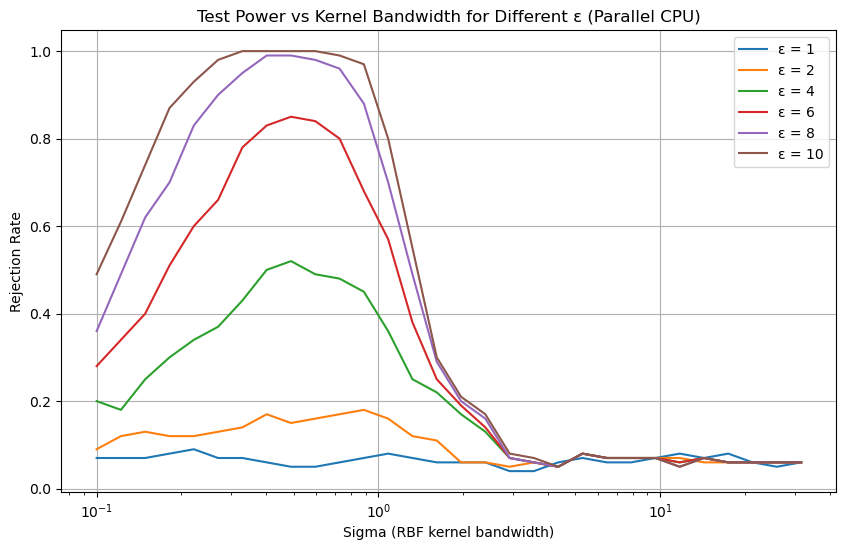
\includegraphics[width=\textwidth]{MMD/Test_powe_vs_eps.png}
    \caption{MMD: Test power vs epsilon shows how well MMD can distinguish between distributions vs how much they differ.}
    \label{fig:mmd_power}
  \end{minipage}
  \hfill
  \begin{minipage}{0.45\textwidth}
    \centering
    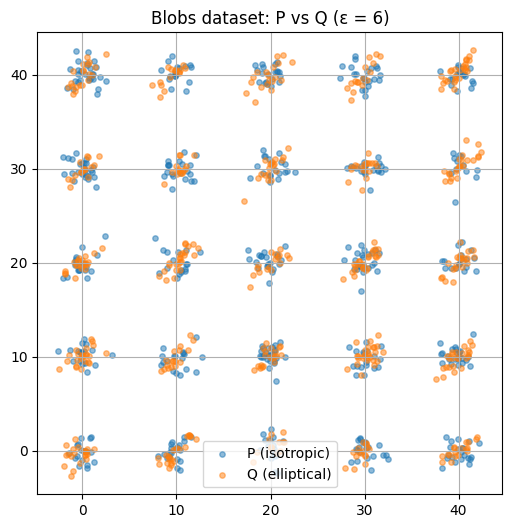
\includegraphics[width=\textwidth]{MMD/Example.png}
    \caption{Example of synthetic dataset used in power calculation.}
    \label{fig:mmd_example}
  \end{minipage}
  

\end{figure}

\subsection{Domain Separation Networks}
\subsubsection{Method}

The key idea is to learn representations that are both \textit{domain-invariant} and \textit{domain-specific}. This is achieved by decomposing the latent representation of an image into two components:
\begin{itemize}
    \item \textbf{Shared representation} (\( h_c \)): Captures features common to both source and target domains.
    \item \textbf{Private representation} (\( h_p \)): Captures features specific to each domain.
\end{itemize}

The model architecture includes:
\begin{itemize}
    \item A \textbf{shared encoder} \( E_c(x) \) for domain-invariant features.
    \item \textbf{Private encoders} \( E_p(x) \) for source and target domains.
    \item A \textbf{shared decoder} \( D(h) \) that reconstructs the input using both private and shared components.
    \item A \textbf{classifier} \( G(h_c) \) trained only on source domain labels.
\end{itemize}

A coarse skeleton of the architectures used in DSNs is shown in \ref{fig:dsn_arch}.

\begin{figure}[h]
  \centering
  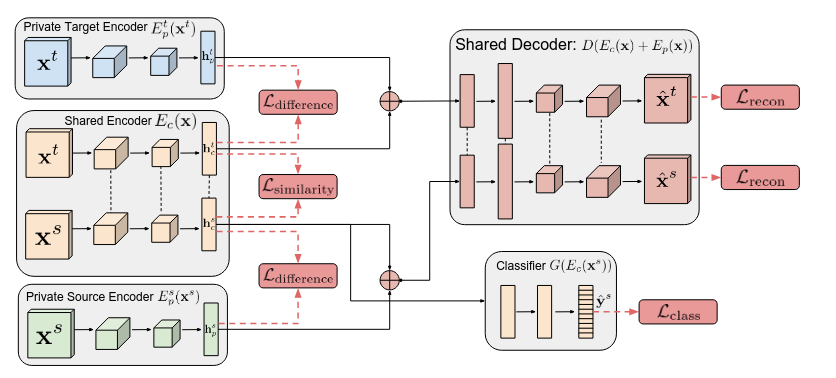
\includegraphics[width=0.8\textwidth]{images/DSN/DSN_arch.png}
  \caption{A coarse skeleton of Domain Separation Networks (DSNs). The architecture separates each input into a domain-specific (private) and domain-invariant (shared) representation. The shared decoder reconstructs the input from both components, while the classifier operates only on the shared features. Learning is guided by four objectives: classification loss (\(\mathcal{L}_{\text{class}}\)), reconstruction loss (\(\mathcal{L}_{\text{recon}}\)), similarity loss (\(\mathcal{L}_{\text{similarity}}\)), and difference loss (\(\mathcal{L}_{\text{difference}}\)).}
  \label{fig:dsn_arch}
\end{figure}

\subsubsection{Learning}

The learning objective is composed of four loss terms:

\begin{equation}
\mathcal{L} = \mathcal{L}_{\text{task}} + \alpha \mathcal{L}_{\text{recon}} + \beta \mathcal{L}_{\text{difference}} + \gamma \mathcal{L}_{\text{similarity}}
\end{equation}

\begin{itemize}
    \item \textbf{Task loss} (\( \mathcal{L}_{\text{task}} \)): Cross-entropy classification loss on the source domain.
    \item \textbf{Reconstruction loss} (\( \mathcal{L}_{\text{recon}} \)): Scale-invariant MSE between the input and reconstruction.
    \item \textbf{Difference loss} (\( \mathcal{L}_{\text{difference}} \)): Enforces orthogonality between shared and private representations using Frobenius norm:
    \[
    \mathcal{L}_{\text{difference}} = \| H_c^s{}^{\top} H_p^s \|_F^2 + \| H_c^t{}^{\top} H_p^t \|_F^2
    \]
    \item \textbf{Similarity loss} (\( \mathcal{L}_{\text{similarity}} \)): Encourages shared representations from both domains to be similar. Two approaches are used:
    \begin{itemize}
        \item \textit{Domain-Adversarial Neural Network (DANN)}: Uses a gradient reversal layer to confuse a domain classifier.
        \item \textit{Maximum Mean Discrepancy (MMD)}: Kernel-based distance to align shared feature distributions.
    \end{itemize}
\end{itemize}

The combined learning strategy ensures that the model:
\begin{enumerate}
    \item Learns a domain-invariant representation for classification.
    \item Separates domain-specific features into private encoders.
    \item Can reconstruct inputs for both domains using both representations.
    \item Enables interpretability via visualization of private and shared components.
\end{enumerate}

\subsubsection{Experiments}
We conducted experiments using Domain Invariant Separation Networks with the DANN approach. MNIST and MNIST-M were used as the train(source) and test(target) data respectively. The accuracy of the trained model on the test data was reported along with the reconstructed images of MNIST and MNIST-M through the shared decoder. The architectures for all the encoders, the decoder, and the classifier were reported through the code submission and the video demonstration of the code.



\subsection{Asymmetric Tri-training for Unsupervised Domain Adaptation}
\subsubsection{Theory}
The Asymmetric Tri-training algorithm is a domain adaptation method that leverages multiple classifiers to improve the performance of a model on a target domain. The key idea is to use two classifiers trained on the source domain to generate pseudo-labels for the target domain, and then use these pseudo-labels to train a third classifier. 

The algorithm works in three main steps:

\begin{enumerate}
  \item \textbf{Source Domain Training}: Two classifiers (F1 and F2) are trained on labeled source domain data.
  
  \item \textbf{Pseudo-labeling}: F1 and F2 are used to predict labels for unlabeled target domain data. Only instances where both classifiers agree with high confidence are selected for pseudo-labeling.
  
  \item \textbf{Target Classifier Training}: A third classifier (Ft) is trained on the pseudo-labeled target domain data, incorporating a multi-view loss to ensure consistency between predictions.
\end{enumerate}

Complete Architecture is shown in figure \ref{fig:att_architecture}.

\textbf{Loss Functions:}\\
 The loss function for Source domain training is the cross-entropy loss + multi-view loss:
\[
  \mathcal{L}(\theta_F, \theta_{F_1}, \theta_{F_2}) = \mathcal{L}_{CE}(F_1(x_s), {y}_s) + 
  \mathcal{L}_{CE}(F_2(x_s), {y}_s) + \lambda
  \|W_1^T W_2\|
\]
The loss function for Target domain training is the cross-entropy loss:
\[
  \mathcal{L}(\theta_F, \theta_{F_t}) = \mathcal{L}_{CE}(F_t(x_t), \hat{y}_t)
\]

\begin{figure}
  \centering
  \includegraphics[width=0.8\textwidth]{ATT/ATT_Architecture.png}
  \caption{ATT Architecture: The feature extractor F processes inputs from both domains. F1 and F2 are source-trained classifiers that generate pseudo-labels for training Ft on the target domain.}
  \label{fig:att_architecture}
\end{figure}

\subsubsection{Pseudocode}
\begin{algorithm}[H]
\caption{Asymmetric Tri-training}
\begin{algorithmic}[1]
\STATE \textbf{Input:} Source data $X_s = \{(x_i, t_i)\}_{i=1}^m$, Target data $X_t = \{(x_j)\}_{j=1}^n$
\STATE $X_t^l = \emptyset$ \COMMENT{Initialize labeled target set}
\FOR{$j = 1$ to $iter$}
  \STATE Train $F, F_1, F_2, F_t$ with mini-batch from training set $S$
\ENDFOR
\STATE $N_t = N_{init}$
\STATE $X_t^l = \text{Labeling}(F, F_1, F_2, X_t, N_t)$
\STATE $L = X_s \cup X_t^l$
\FOR{$K$ steps}
  \FOR{$j = 1$ to $iter$}
    \STATE Train $F, F_1, F_2$ with mini-batch from training set $L$
    \STATE Train $F, F_t$ with mini-batch from training set $X_t^l$
  \ENDFOR
  \STATE $X_t^l = \emptyset$, $N_t = K/20 * n$
  \STATE $X_t^l = \text{Labeling}(F, F_1, F_2, X_t, N_t)$
  \STATE $L = X_s \cup X_t^l$
\ENDFOR
\end{algorithmic}
\end{algorithm}

\subsubsection{Implementation Details}
We implemented the Asymmetric Tri-training algorithm using PyTorch. The model architecture (fig\ref{fig:att_implementation}) consists of a feature extractor followed by three classifiers. The feature extractor is a convolutional neural network (CNN) for image data, while the classifiers are fully connected layers. We used momentum SGD with a learning rate of 0.01 and momentum 0.9 and a batch size of 128. Lamda was set to 0.01 for the multi-view loss. We trained for 20 iters and value of K as 50. This computation required 2-3 hours of training time on GPU hence we were not able to train it for the recommened 2000 iterations as mentioned in the paper. Which we believe is the reason for the discrepancy in results as compared to the paper.
\begin{figure}[h]
  \centering
  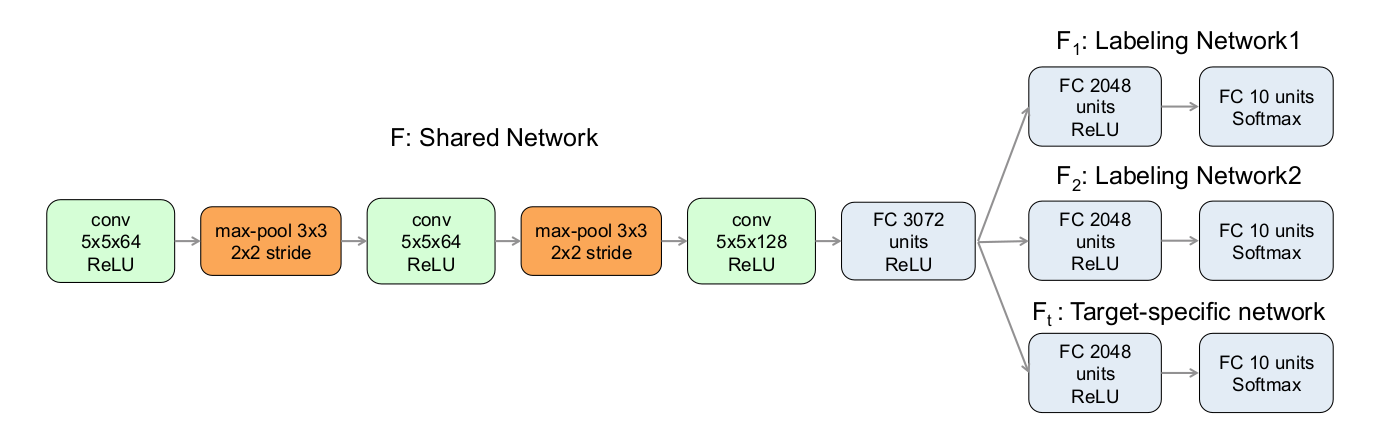
\includegraphics[width=0.8\textwidth]{ATT/Imp_acc.png}
  \caption{Architecture used for SVHN-MNIST domain adaptation. The feature extractor is a CNN with batch normalization in the last convolutional layer, and the classifiers are fully connected layers with batch normalization and dropout.}
  \label{fig:att_implementation}
\end{figure}

\subsection{A Theory of learning from different domains}

\subsubsection{Introduction}
% Expanded introduction, background on domain adaptation
This paper\cite{Ben-David2010} introduces the theoretical framework for domain adaptation, specifcally Supervised Domain Adaptation. This is particularly important in scenarios where labeled data is scarce or expensive to obtain in the target domain, but abundant in the source domain. \\
\\
In many real-world applications, such as image recognition or natural language processing, the performance of machine learning models can degrade significantly when the training and testing data come from different distributions. This phenomenon is known as domain shift or covariate shift. To prevent this, domain adaptation seeks to transfer knowledge from the source to the target domain effectively via the learning of \textbf{domain independent features} of source dataset.
\\
\\
The $\mathcal{H}$-divergence is a measure of the difference between two probability distributions. Such a measure is important as it helps us quanitfy how different 2 distributions are from each other. We will first derive an upper bound over $\mathcal{H}$-divergence between the source and target domain. After that we will try to estimate an optimal value of $\alpha$ which is a parameter that controls the trade-off between the source and target domain errors. The goal is to minimize the source error while ensuring that the model generalizes well to the target domain. We will also provide a theoretical analysis of the alpha-error bound, which quantifies the relationship between the source and target domain errors.

\subsection{Problem Formulation}
We formalize the problem of domain adaptation for binary classification as follows. A domain is defined to be a pair of a distribution $D$ over inputs $X$ and a labeling function $f : X \to [0,1]$, which can take fractional (expected) values when labeling occurs non-deterministically. Initially, we will consider two domains: a source domain and a target domain. 

We denote the source domain by $(D_S, f_S)$ and the target domain by $(D_T, f_T)$. A hypothesis is a function $h : X \to \{0,1\}$ which labels the inputs. The probability that a hypothesis $h$ disagrees with a labeling function $f$ (which can also be a hypothesis) when evaluated over a distribution $D_S$ is defined as follows:
\[
\epsilon_S(h, f) = \mathbb{E}_{x \sim D_S} \big[ |h(x) - f(x)| \big].
\]

When referring to the source error (sometimes called risk) of a hypothesis, we use the shorthand notation:
\[
\epsilon_S(h) = \epsilon_S(h, f_S).
\]

\subsubsection{Notation and Definitions}
\begin{definition}
    Given a domain $X$ with distributions $D_1$ and $D_2$ over $X$, let $\mathcal{H}$ be a hypothesis class on $X$. For any hypothesis $h \in \mathcal{H}$, denote by $I(h)$ the set of points for which $h$ is the characteristic function, i.e., $x \in I(h) \iff h(x) = 1$. The $H$-divergence between $D_1$ and $D_2$ is defined as:
    \[
    d_{\mathcal{H}}(D_1, D_2) = 2 \sup_{h \in \mathcal{H}} \big| \Pr_{x \sim D_1}[x \in I(h)] - \Pr_{x \sim D_2}[x \in I(h)] \big|.
    \]
\end{definition}
The advantage of using $H$-divergence over other metrics is due to the relative ease in estimating its upper bound in terms of empirical values. 
\\
\\
Consider the case of the hypothesis class being of finite VC dimension and is symmetric. Following are certain lemmas which will help us in estimating the upper bound of the $\mathcal{H}$-divergence. 
\\
\\
\begin{lemma}
Let $\mathcal{H}$ be a hypothesis space on $X$ with VC dimension $d$. If $U$ and $U'$ are samples of size $m$ from $D_1$ and $D_2$ respectively, and $\hat{d}_{\mathcal{H}}(U, U')$ is the empirical $H$-divergence between the samples, then for any $\delta \in (0,1)$, with probability at least $1 - \delta$, the following holds:
\[
d_{\mathcal{H}}(D_1, D_2) \leq \hat{d}_{\mathcal{H}}(U, U') + 4 \sqrt{\frac{d \log(2m) + \log\left(\frac{2}{\delta}\right)}{m}}.
\]
\end{lemma}
This Lemma shows that the empirical $\mathcal{H}$-divergence between two samples from distributions
$D_1$ and $D_2$ converges uniformly to the true $\mathcal{H}$-divergence for hypothesis classes $\mathcal{H}$ of finite VC dimension.
\begin{lemma}
For a symmetric hypothesis class $\mathcal{H}$ (one where for every $h \in \mathcal{H}$, the inverse hypothesis $1 - h$ is also in $\mathcal{H}$) and samples $U, U'$ of size $m$, the empirical $H$-divergence is given by:
\[
\hat{d}_{\mathcal{H}}(U, U') = 2 \left( 1 - \min_{h \in \mathcal{H}} \left[ \frac{1}{m} \sum_{x : h(x) = 0} \mathbb{I}[x \in U] + \frac{1}{m} \sum_{x : h(x) = 1} \mathbb{I}[x \in U'] \right] \right),
\]
where $\mathbb{I}[x \in U]$ is the binary indicator variable, which is $1$ when $x \in U$ and $0$ otherwise.
\end{lemma}
This lemma directly motivates a procedure for computing the $\mathcal{H}$-divergence.

\begin{definition}
The ideal joint hypothesis is the hypothesis which minimizes the combined error:
\[
h^* = \arg\min_{h \in \mathcal{H}} \big(S(h) + T(h)\big).
\]
We denote the combined error of the ideal hypothesis by:
\[
\lambda = S(h^*) + T(h^*).
\]
\end{definition}
This $\lambda$ will be used in our analysis of the alpha-error bound.\\
Now, let's define a term called \textbf{Symmetric Difference Hypothesis Space} which is a very crucial for our further analysis.\\
\begin{definition}
For a hypothesis space $\mathcal{H}$, the symmetric difference hypothesis space $\mathcal{H} \Delta \mathcal{H}$ is
the set of hypotheses
\[
g \in \mathcal{H} \Delta \mathcal{H} \iff g(x) = h_1(x) \oplus h_2(x) \text{ for some } h_1, h_2 \in \mathcal{H},
\]
where $\oplus$ is the XOR function. In words, every hypothesis $g \in \mathcal{H} \Delta \mathcal{H}$ is the set of disagreements
between two hypotheses in $\mathcal{H}$.
\end{definition}

The below lemma will give us an idea on how to incorporate this symmetric difference hypothesis space in our analysis.\\
\begin{lemma}
    For any hypotheses $h_1, h_2 \in \mathcal{H}$, the following inequality holds:
    \[
    | \epsilon_S(h_1, h_2) - \epsilon_T(h_1, h_2) | \leq \frac{1}{2} d_{\mathcal{H}\Delta \mathcal{H}}(D_S, D_T)
    \]
\end{lemma}
\\ 
The following theorem can be easily proved using the above lemma:
\\
\\
\begin{theorem}
\textit{Let $\mathcal{H}$ be a hypothesis space of VC dimension $d$. If $\mathcal{U}_S, \mathcal{U}_T$ are unlabeled samples of size $m'$ each, drawn from $\mathcal{D}_S$ and $\mathcal{D}_T$ respectively, then for any $\delta \in (0, 1)$, with probability at least $1 - \delta$ (over the choice of the samples), for every $h \in \mathcal{H}$:}
\[
\epsilon_T(h) \leq \epsilon_S(h) + \frac{1}{2} \hat{d}_{\mathcal{H} \Delta \mathcal{H}}(\mathcal{U}_S, \mathcal{U}_T) + 4 \sqrt{\frac{2d \log(2m') + \log\left(\frac{2}{\delta}\right)}{m'}} + \lambda.
\]
\end{theorem}
Now, let's denote our loss as:
\[
\hat{\epsilon_\alpha}(h) = \alpha \hat{\epsilon_T}(h) + (1-\alpha) \hat{\epsilon_S}(h)
\]
where $\alpha \in [0,1]$. We want to find the optimal $\alpha$ such that the target loss is as low as possible.
 \\
The following lemmas are essential in calculating the optimal value of $\alpha$
 \\ \\
 \textbf{Lemma 4} \textit{Let $h$ be a hypothesis in class $\mathcal{H}$. Then}
\[
|\epsilon_\alpha(h) - \epsilon_T(h)| \leq (1 - \alpha) \left( \frac{1}{2} d_{\mathcal{H} \Delta \mathcal{H}}(\mathcal{D}_S, \mathcal{D}_T) + \lambda \right).
\]
\\
The lemma shows that as $\alpha$ approaches 1, we rely increasingly on the target data, and the distance between domains matters less and less.

\begin{lemma}[Lemma 5]
For a fixed hypothesis $h$, if a random labeled sample of size $m$ is generated by drawing $\beta m$ points from $D_T$ and $(1 - \beta)m$ points from $D_S$, and labeling them according to $f_S$ and $f_T$ respectively, then for any $\delta \in (0,1)$, with probability at least $1 - \delta$ (over the choice of the samples),
\[
\Pr\left[|\hat{\varepsilon}_\alpha(h) - \varepsilon_\alpha(h)| \geq \epsilon \right] \leq 2 \exp\left(-2m\epsilon^2 \left/ \left( \frac{\alpha^2}{\beta} + \frac{(1 - \alpha)^2}{1 - \beta} \right) \right.\right).
\]
\end{lemma}

It can easily be proved using Hoeffding’s inequality.

\begin{proposition}[Hoeffding’s inequality]
If $X_1, \ldots, X_n$ are independent random variables with $a_i \leq X_i \leq b_i$ for all $i$, then for any $\epsilon > 0$,
\[
\Pr\left[|\bar{X} - \mathbb{E}[\bar{X}]| \geq \epsilon\right] \leq 2 \exp\left(-\frac{2n^2\epsilon^2}{\sum_{i=1}^n (b_i - a_i)^2} \right),
\]
where $\bar{X} = \frac{1}{n} \sum_{i=1}^n X_i$.
\end{proposition}
\\

\begin{theorem}
Let $\mathcal{H}$ be a hypothesis space of VC dimension $d$. Let $U_S$ and $U_T$ be unlabeled samples of size $m'$ from $D_S$ and $D_T$, respectively. Let $S$ be a labeled sample of size $m$, with $\beta m$ from $D_T$ and $(1 - \beta)m$ from $D_S$, labeled by $f_T$ and $f_S$, respectively.

If $\hat{h} \in \mathcal{H}$ is the empirical minimizer of $\hat{\varepsilon}_\alpha(h)$ on $S$, and $h_T^* = \arg\min_{h \in \mathcal{H}} \varepsilon_T(h)$, then for any $\delta \in (0, 1)$, with probability at least $1 - \delta$:
\begin{align*}
\varepsilon_T(\hat{h}) \leq & \ \varepsilon_T(h_T^*) + 4 \sqrt{\frac{\alpha^2}{\beta} + \frac{(1 - \alpha)^2}{1 - \beta}} \cdot \sqrt{\frac{2d \log(2(m + 1)) + 2 \log(8 / \delta)}{m}} \\
& + 2(1 - \alpha) \left( \frac{1}{2} \hat{d}_{\mathcal{H} \Delta \mathcal{H}}(U_S, U_T) + 4 \sqrt{\frac{2d \log(2m') + \log(8 / \delta)}{m'}} + \lambda \right).
\end{align*}
\end{theorem}

This theorem can be easily proved using the last 3 lemmas.

\subsection*{Optimal Mixing Value}

Let us define:
\[
f(\alpha) = 2B \sqrt{\frac{\alpha^2}{\beta} + \frac{(1 - \alpha)^2}{1 - \beta}} + 2(1 - \alpha)A,
\]
where
\[
A = \frac{1}{2} \hat{d}_{\mathcal{H} \Delta \mathcal{H}}(U_S, U_T) + 4 \sqrt{\frac{2d \log(2m') + \log(4/\delta)}{m'}} + \lambda,
\quad
B = 4 \sqrt{\frac{2d \log(2(m + 1)) + 2 \log(8/\delta)}{m}}.
\]

Define $D = \sqrt{d}/A$. Then the optimal value $\alpha^*$ is:
\[
\alpha^*(m_T, m_S; D) = 
\begin{cases}
1 & \text{if } m_T \geq D^2, \\
\min\{1, \nu\} & \text{otherwise},
\end{cases}
\]
where
\[
\nu = \frac{m_T}{m_T + m_S} \left(1 + \frac{m_S}{\sqrt{D^2(m_S + m_T) - m_S m_T}}\right).
\]

\subsubsection{Conclusion}
In conclusion, this paper introduced the theoretical framework for supervised domain adaptation. While training, we will assign different weights to the losses of the two domains: source and target. The paper illustrates the factors on which the optimal weight value where the optimal weight value refers to the weight producing the lowest combined error. This weight in general depends on $\beta$, VC dimension and the number of training points.

\section*{Acknowledgements}
We would like to express our sincere gratitude to Prof. Chiranjib Bhattacharyya and Prof. Shishir N. Y. Kolathaya for offering the course UMC203, which provided us with a strong foundation that greatly helped us in the preparation of this report. We are especially thankful to our TA, Pranav K. Nayak, for his guidance, prompt support, and constructive feedback throughout the project. This project would not have been possible without the intellectually stimulating environment fostered by the instructors and the TA.

\section*{Contributions}
\textbf{Pratham Gupta:}
\begin{itemize}
    \item Codes for MMD and ATT algorithms
    \item Complete Main Section of Report 
    \item MMD and ATT in Appendix Section of Report
    \item Presentation Slides of Introduction, DSN, MMD and ATT
    \item Video Editing 
    \item Maintained Repository of the project
    \item Worked on DANN Re-identification Code
\end{itemize}
\textbf{Gavish Bansal:}
\begin{itemize}
    \item Codes for Sentiment Analysis and Re identification Code
    \item Complete Appendix Section of DANN and Theory paper in Report 
    \item Prepared Presentation for DANN part
\end{itemize}
\textbf{Kintan Saha:}
\begin{itemize}
    \item Code for the inter-twined moons setup.
    \item Code for image classification experiments of the DANN paper.
    \item Writing the Appendix section for the DANN paper and the theory paper.
    \item Helping in preparing the presentation slides for the DANN part.
\end{itemize}
\textbf{Krishna Agarwal}
\begin{itemize}
    \item Codes for CORAL, DeepCORAL, and DSN.
    \item Helped in writing sections of CORAL, DeepCORAL, and DSN in the main report.
    \item Writing the Appendix section for the Survey paper.
    \item Presentation slides for CORAL and DeepCORAL.
\end{itemize}


% \section*{References}
\bibliographystyle{unsrt}
\bibliography{references}

%%%%%%%%%%%%%%%%%%%%%%%%%%%%%%%%%%%%%%%%%%%%%%%%%%%%%%%%%%%%


\end{document}